\documentclass[12pt,letterpaper]{article}

% --- Preamble ---
% manuscript-preamble.tex — Chicago Author-Date manuscript preamble
% Shared preamble for manuscript and potential slide reuse

% --- Fonts ---
% Support both PdfLaTeX and Xe/LuaLaTeX.
\usepackage{iftex}
\ifPDFTeX
  \usepackage[T1]{fontenc}
  \usepackage[utf8]{inputenc}
  \usepackage{newtxtext}
  \usepackage{newtxmath}
\else
  \usepackage{fontspec}
  \setmainfont{Times New Roman}[Ligatures=TeX]
\fi

% --- Layout ---
\usepackage[margin=1in]{geometry}
\usepackage{setspace}
\doublespacing

% --- Math & symbols ---
\usepackage{amsmath}
\ifPDFTeX
  % newtxmath already provides most AMS-style symbols under PdfLaTeX
\else
  \usepackage{amssymb}
\fi

% --- Tables ---
\usepackage{booktabs}
\usepackage{tabularx}
\usepackage{longtable}
\usepackage{multirow}
\usepackage{array}
\usepackage{dcolumn}

% --- Figures ---
\usepackage{graphicx}
\usepackage{float}

% --- Citations (Chicago Author-Date via biblatex-chicago) ---
% Compile: xelatex -> biber -> xelatex -> xelatex
\usepackage[
  authordate,
  backend=biber,
  natbib=true,
  url=true,
  doi=true,
  isbn=false
]{biblatex-chicago}
\addbibresource{references.bib}

% --- Cross-references & links ---
\usepackage{hyperref}
\hypersetup{
  colorlinks=true,
  linkcolor=black,
  citecolor=black,
  urlcolor=blue,
  pdfauthor={},
  pdftitle={Issue-Bounded Conditionality in U.S. Public Opinion on Fentanyl Policy}
}

% --- Appendix support ---
\usepackage[toc,page]{appendix}

% --- Landscape pages for wide tables ---
\usepackage{pdflscape}

% --- Misc ---
\usepackage{enumerate}
\usepackage{etoolbox}
\usepackage{caption}
\captionsetup{font=small,labelfont=bf,hypcap=false}

% --- Prevent doublespacing inside tables ---
\AtBeginEnvironment{tabular}{\singlespacing}
\AtBeginEnvironment{longtable}{\singlespacing}

% --- Reduce noisy line-breaking diagnostics ---
\hbadness=10000
\hfuzz=200pt


\vbadness=10000
\vfuzz=500pt


% --- Cross-document references to online Supplementary Material ---
\usepackage{xr-hyper}
\externaldocument{supplementary}

% --- Metadata ---
\title{When Warm Feelings Harden: Fentanyl Crisis Blame and U.S. Public Opinion on China}
\author{
  Junyang Hu\thanks{PAX \textit{sapiens} Foundation. Corresponding author: \texttt{jhu@paxsapiens.org}.}
}
\date{\today}

\begin{document}

\maketitle
\thispagestyle{empty}

% ===========================================================================
% ABSTRACT
% ===========================================================================
\begin{abstract}
\noindent \singlespacing

How do Americans form policy preferences toward China when a domestic crisis is externally attributed? Drawing on two nationally representative surveys of U.S. adults fielded in 2024 and 2025, this article introduces the concept of issue-bounded conditionality: the coexistence of coercive and cooperative policy preferences within a single issue domain without extending across areas. Warmth toward China and blame for the fentanyl crisis jointly shape both generalized bilateral posture and issue-level tool preferences, but these two levels of opinion do not move in lockstep. Among respondents who continue to hold relatively warmer views of China, blame is associated with a sanctions-and-cooperation configuration instead of a uniformly confrontational stance. A specificity test spanning eight policy domains shows that this pattern is concentrated in the fentanyl domain, with little evidence of spillover to areas such as cross-Strait tension, economic decoupling, or educational exchange. These findings show that support for issue-specific engagement is most durable when tied to a concrete, accountable objective rather than to abstract appeals to goodwill.

\end{abstract}

\noindent \textbf{Keywords:} U.S.-China relations, public opinion, crisis blame, issue-bounded conditionality

\newpage
\setcounter{page}{1}

% ===========================================================================
% 1. INTRODUCTION
% ===========================================================================
\section{Introduction}
\label{sec:introduction}

Over the past decade, claims that China poses a threat to U.S. national interests and to the liberal international order have structured much of Washington's debate on China, though the precise framing has varied across administrations. One policy domain in which these shifts have had direct and tangible consequences is the U.S. synthetic opioid epidemic. The crisis reaches into nearly every community: nearly one-third of Americans report that they or a family member have experienced opioid addiction, and about one-fifth report knowing someone who died of an overdose \citep{hu_blame_2025,saunders_opioid_2026}. Fentanyl, a synthetic opioid responsible for over half of U.S. overdose deaths since 2019 and nearly 70\% of such deaths in 2023, now exemplifies a transnational public health emergency with geopolitical underpinnings \citep{usafacts_are_2025}. The People's Republic of China (PRC) has been identified as a primary source of precursor chemicals used in the illicit production of fentanyl by Mexican cartels. 

Despite Beijing's 2019 regulatory measures to curb fentanyl-related exports, U.S. politicians and pundits have increasingly characterized the PRC's role as ranging from negligent to deliberately exploitative, with some describing the flow of precursor chemicals as an ``asymmetric weapon'' \citep{martinez-fernandez_holding_2024}. In a 2024 report, the House Select Committee on the Chinese Communist Party concluded that the PRC government subsidizes the manufacture and export of illicit fentanyl materials and other synthetic narcotics, fails to prosecute major traffickers, permits open online sales of precursor chemicals, and derives strategic and economic benefit from the crisis \citep{us_house_select_committee_on_the_strategic_competition_between_the_united_states_and_the_chinese_communist_party_ccps_2024}. These assessments, in turn, have helped drive congressional proposals to broaden sanctionable categories and designate certain Chinese entities and officials as ``foreign opioid traffickers'' \citep{barr_hr747_2025}. 

The executive branch, for its part, has likewise highlighted the growing role of Chinese money-laundering networks in facilitating the operations of Mexico-based transnational criminal organizations (TCOs). Beginning in 2025, the Trump administration folded this line of argument into a broader national-security narrative that portrayed China as an ``unusual and extraordinary threat'' and as a source of support and safe haven for fentanyl-linked TCOs \citep{the_white_house_imposing_2025}. Together, these developments translated into concrete policy, from the imposition of fentanyl-related tariffs in early 2025 to a bilateral presidential agreement in Busan later that year. In doing so, Washington has embraced a model of transactional \textit{realpolitik} that ties punitive tariffs and technology export controls to stepped-up counternarcotics enforcement.

Although the terms of both Washington's political debate and its dealings with Beijing have been reshaped, elite-level shifts do not by themselves explain how ordinary Americans translate blame for the opioid crisis into their foreign-policy preferences. Whether ordinary citizens engage in a similar form of transactional reasoning and under what conditions remains an open question. Elite cues on China are often contradictory---simultaneously framing Beijing as a partner in counternarcotics cooperation and as a deliberate enabler of the crisis---and citizens bring their own affective dispositions and issue-specific judgments to bear. Public attitudes toward China remain broadly negative, yet they are far from monolithic. The share describing China as an outright ``enemy'' fell from 42\% to 33\% in a single year, and for the first time since 2019, a majority of Americans favored ``friendly cooperation and engagement'' with Beijing \citep{huang_negative_2025, kafura_americans_2025}. The Chicago Council on Global Affairs annual surveys \citep{kafura_americans_2025} provide the closest national-benchmark comparator for these trends in U.S. attitudes toward China; the 2024--2025 waves analyzed here track the Chicago Council figures on aggregate warmth and cooperation support within 3 percentage points while adding the granularity to decompose tool configurations. Such aggregate figures mask considerable internal differentiation: Americans can hold negative general impressions of a foreign country while supporting cooperation on specific issues, and favorability ratings and policy-domain preferences do not always move in tandem \citep{holsti_public_2004, gries_political_2010, jin_americans_2021}. More than a thermometer of bilateral tensions, public opinion functions as an independent source of constraint and legitimation in foreign-policy formation.

How this differentiated structure operates when a lethal domestic crisis is attributed to a foreign rival is the puzzle this article addresses. Blame, threat perception, and potential cooperation are unusually intertwined in the fentanyl case. The resulting opinion dynamics cannot be adequately captured by a single hawk--dove dimension: affective warmth toward China, support for coercive policy tools, and responsiveness to crisis cues need not lie on a single continuum. This premise thus motivates two related questions. First, does the relationship between warmth and foreign-policy posture hold, intensify, or collapse into uniform confrontation when China is blamed for a serious domestic harm? Second, can warmth coexist with endorsement of coercive instruments---and if so, is this coexistence domain-specific or does it generalize across policy areas? Answering these questions requires examining whether crisis blame suppresses, reverses, or reorganizes the relationship between warmth and coercive preferences.

To that end, the article draws on two nationally representative YouGov survey waves in 2024 and 2025. The findings reveal a conditional rather than linear relationship. Warmth toward China is associated with a more dovish general posture, and this association is not eliminated by blaming China for the fentanyl crisis. Among respondents who view China warmly, blame is not associated with a uniform shift toward punishment. Instead, blame is associated with a distinctive mixed configuration---pairing coercive pressure with demands for cooperative engagement---rather than with sanctions alone. An eight-probe specificity test, using seven boundary probes as a negative-control exercise, further confirms that this pattern is domain-specific. The coexistence of warmth and coercive support appears in the fentanyl-cooperation scenario and is largely absent in military, economic, and cultural domains. Warmth toward China coexists with support for coercive instruments when those instruments are tied to a concrete, reciprocal, and issue-specific form of cooperation.

The findings speak to three literatures. The image-theory tradition treats national images as structured by broad relational variables---relative power, perceived threat, cultural status---not issue-specific attributions \citep{herrmann_images_1997}. Blame intensifying cooperative preferences among those who view China favorably demonstrates that issue-specific cognitions can redirect, not merely reinforce, the policy consequences of affect. The article also draws a distinction between general posture and instrument choice that is undertheorized in research on economic statecraft. Building on evidence that citizens evaluate sanctions instrumentally, weighing expected consequences rather than expressing generalized hostility \citep{jentleson_pretty_1992, heinrich_sanction_2017}, the results show that preferences for coercive tools can coexist with a cooperative orientation when those tools are perceived as serving a specific bargaining objective. Finally, the article extends research on ``issue publics''---subgroups with unusually structured attitudes on salient matters---to the foreign-policy instrument domain \citep{krosnick_government_1990, krosnick_public_1995}. Recent work theorizes that such publics form when a pivotal circumstance activates the political relevance of a latent group characteristic \citep{rossiter_development_2026}. That warmth-plus-coercion preferences toward China are confined to the fentanyl scenario is consistent with this logic: crisis blame is associated with issue-bounded preference structures that cut across the conventional hawk--dove continuum.

Section~\ref{sec:theory} reviews the relevant literature and develops the theoretical framework. Section~\ref{sec:data} introduces the data, measures, and analytical strategy. Section~\ref{sec:results} presents the empirical findings, moving from general posture (Section~\ref{sec:results_posture}) to tool configuration (Section~\ref{sec:results_toolconfig}) and the scenario-based specificity test (Section~\ref{sec:results_specificity}). Section~\ref{sec:discussion} discusses implications for the study of U.S.-China relations and democratic foreign-policy formation.

% ===========================================================================
% 2. THEORETICAL FRAMEWORK
% ===========================================================================
\section{Literature and Theory}
\label{sec:theory}

% ¶1 — Layer 1: Threat-Affect-Elite Baseline
\subsection{From Threat Perception to Issue-Level Reasoning}
\label{sec:theory_literature}

When domestic crises intersect with foreign actors, threat perception and emotional arousal should dominate public reasoning about foreign policy. Appraisal theories of emotion hold that anger and fear---discrete affective states triggered by perceived threat---generate systematically different risk assessments and policy preferences \citep{marcus_affective_2000, lerner_fear_2001, herrmann_how_2017, renshon_emotions_2017}. In the foreign policy domain, anxiety sometimes prompts risk aversion and impairs cognitive performance, while anger fosters a desire for retributive punishment that can override established partisan leanings \citep{brader_what_2008, huddy_threat_2005, wayne_terrified_2023}. In cases of high-stakes conflict, reminders of external aggression often lead to increased support for hardline policies regardless of whether the specific emotion felt is fear or anger \citep{kupatadze_shadow_2021}. Similarly, when citizens perceive a foreign actor as both powerful and threatening, adversary-image schemata can also activate, channeling preferences toward confrontation \citep{herrmann_mass_1999}. Elite cues reinforce these tendencies. When bipartisan consensus narrows the available frames---as has occurred with ``tough on China'' rhetoric in U.S. politics---the cue space constricts, and citizens face few elite signals that might encourage more differentiated reasoning \citep{zaller_nature_1992}. Together, these frameworks predict a unidimensional hawkish shift. The more negative the affect toward the rival, the more confrontational the public's preferences should be across all policy dimensions. Yet this prediction sits uneasily with a recurrent empirical pattern. Some citizens simultaneously endorse punitive measures \emph{and} domain-specific cooperation with the same adversary---a configuration that purely affect-driven models do not capture.

% ¶2 — Layer 2: Bottom-Up Correction
While these frameworks powerfully explain the general hawkish tilt in crisis contexts, they predict a uniformity of response that the empirical record increasingly contradicts. Even within the elite-cueing tradition, recent work shows that cue effects weaken when citizens possess independent policy information or when partisan polarization channels processing through pre-existing attitudes over elite frames \citep{bullock_elite_2011, guisinger_mapping_2017}. A more fundamental challenge comes from research demonstrating that public foreign policy attitudes are not volatile reactions to elite signals but hierarchically organized belief systems in which general orientations---rooted in values, dispositions, and social identifications---constrain more specific policy preferences \citep{hurwitz_how_1987}. Citizens form coherent foreign policy attitudes even without elite guidance, suggesting that preference structures are built from the bottom up rather than imposed from the top down \citep{kertzer_bottom-up_2017}. The same basic personal values that guide daily choices also structure foreign-policy orientations: conservation values predict militant internationalism while universalism predicts cooperative internationalism, a pattern that holds even among low-knowledge respondents \citep{rathbun_taking_2016}. Across decades and issue domains, aggregate public opinion exhibits a degree of stability and internal coherence that cannot be reduced to a simple hawk--dove continuum \citep{page_rational_1992, kertzer_public_2023}. 

This multidimensionality is visible in the U.S.-China case too, where public attitudes are constructed beyond a single favorable--unfavorable metric \citep{li_more_2021}. Despite bipartisan consensus that China ``dodges'' international responsibility based on its domestic governance and strategic weight, ideology and partisanship produce sharp cleavages over China policy \citep{gries_political_2010, gries_red_2014, li_how_2015}. The pattern sharpens when specific policy domains are examined. Americans can simultaneously view bilateral trade as beneficial and endorse the trade war as legitimate, with the two judgments driven by distinct factors---general trade attitudes shaped by cultural perceptions of China, trade-war support predicted primarily by partisan identification \citep{jin_americans_2021}. The coexistence has limits, though. Experimental data suggests that perceived economic opportunity improves American attitudes toward democratic partners but fails to moderate hostility toward authoritarian states, where judgments of China's political culture dominate \citep{wick_capabilities_2014}. Attitudes are structured and internally differentiated. But structure along what dimensions? Specifically, is the relevant structure organized around the \emph{objectives} of foreign policy action, the \emph{instruments} through which action is applied, or the \emph{issue domains} on which action is taken? The ``structured opinion'' finding opens this dimensionality question without answering it.

% ¶3 — Layer 3: Policy-Objectives Correction (PPO)
One influential answer identifies the principal policy objective (PPO) as the primary axis of differentiation. Jentleson's ``pretty prudent public'' thesis demonstrated that American support for the use of military force varies systematically by the stated objective of intervention. Restraining an external aggressor or humanitarian intervention both receive substantially higher support than internal political change \citep{jentleson_pretty_1992, jentleson_still_1998}. This objective-sensitivity proved robust across the post-Cold War period, surviving changes in threat environment and partisan alignment. More recent work extends the insight beyond military force to economic statecraft, showing that citizens' trade preferences are shaped by geopolitical alignment with trading partners---preferring allies over adversaries due to security concerns---rather than being determined solely by material self-interest \citep{carnegie_public_2022}. The public applies conditional judgment based on the perceived purpose of foreign policy action, not a blanket hawkish or dovish disposition. Yet the PPO framework, for all its explanatory power, implicitly treats alternative instruments as interchangeable means to a shared end. A citizen who endorses ``restraining an aggressor'' may nonetheless evaluate sanctions, diplomatic pressure, and military action very differently---even when all three serve the same objective. Whether citizens treat instruments as interchangeable conditional on endorsing a given objective remains underspecified.

% ¶4 — Layer 4: Instruments and Relational Coercion
Recent work on public support for specific coercive tools suggests they do not. Even holding objectives constant, instruments carry independent weight in public evaluation. A growing experimental literature examines the conditions under which mass publics support coercive versus cooperative instruments in bilateral relationships \citep{tomz_domestic_2007, tomz_public_2013, heinrich_sanction_2017, frye_economic_2019}. Survey-experimental evidence shows that citizens support sanctions more when they expect the measures to deter future misbehavior by the target state; support declines as anticipated domestic economic costs to the sender increase \citep{heinrich_sanction_2017}. Related work shows that human rights framing and target-population salience further condition public support for sanctions, with tailored sanctions targeting leadership tending to attract greater backing than comprehensive ones \citep{mclean_public_2017, ari_human_2025}. Built upon evidence that citizens also differentiate tools by objective \citep{levin_what_2025}, this article argues that instruments carry not only cost-benefit weight but different relational meanings. The observational design complements the experimental literature by showing how warmth and blame jointly reshape tool-configuration preferences outside the experimental frame. Some tools are read as punitive, relationship-ending signals, while others are interpreted as relationship-managing ones---compliance-seeking leverage deployed within an ongoing engagement. The literature has begun to document this distinction but has not yet specified when and for whom the relational framing applies, nor has it clearly theorized why citizens would combine punitive and cooperative tools simultaneously on a single issue—the question this article takes up.

% ¶5 — Layer 5: Issue Publics — Scope Narrowing
These findings raise a scope question: if such differentiated reasoning exists, does it characterize the general public, or a specific subset of citizens for whom the issue is especially salient? Krosnick's issue-publics framework provides the relevant boundary condition. Citizens vary in the personal importance they attach to particular policy issues. Those for whom an issue is highly important form an ``issue public'' marked by greater attitude stability and heightened political engagement on that issue \citep{krosnick_attitude_1989, krosnick_government_1990, krosnick_public_1995}. Issue-bounded conditionality builds on this accessibility-importance tradition: high-importance issues are cognitively structured and chronically accessible, a property that permits blame-driven conditionality to organize preferences within the issue domain without propagating to adjacent issues. Issue publics are not fixed demographic categories but form dynamically through a two-stage process. Groups with latent connections to a political issue constitute potential issue publics until a pivotal circumstance personalizes the issue's political relevance for individual members \citep{rossiter_development_2026}. By this logic, the fentanyl crisis---personally salient for millions of affected families and newly politicized through attribution to China---may have activated precisely this kind of domain-specific attentive constituency. The concept matters here not only because it helps identify who engages in differentiated reasoning, but also because it suggests why issue domains themselves may become independent axes of preference formation. When an issue commands sustained personal importance, it can generate a distinct attitudinal space, organized around that domain's specific objectives and instruments, one not reducible to general foreign policy posture. If so, the differentiated reasoning documented in the preceding literature is more likely to appear among those for whom the fentanyl crisis is personally salient than across the mass public uniformly.

Existing work therefore suggests that foreign-policy attitudes are organized across distinct objects of judgment. Citizens who are attentive to a given issue may form views about the bilateral relationship as a whole \emph{and} separate views about the appropriate instrument for handling a particular dispute within that relationship. The literature has not theorized how these two levels interact---nor what conditions enable citizens to hold both punitive and cooperative preferences simultaneously. The following conceptual framework addresses this question.

% ¶6 — Theory Construction Block (Part 1): Analytical Levels + Mechanism
\subsection{Issue-Bounded Conditionality: A Conceptual Framework}
\label{sec:theory_ibc}

This article advances two related claims. The first is structural: foreign-policy attitudes toward a rival state operate at more than one analytical level, and under some crisis conditions these levels can come apart. The second is conditional: this decoupling is not uniform across issues but occurs only where specific scope conditions are met. The resulting pattern is termed \emph{issue-bounded conditionality}---the coexistence of domain-specific coercive support with cooperative engagement on the same issue, in a manner that does not generalize across policy domains. The two claims are logically separable and face different counterarguments, and this article develops them in turn.

\textit{Two levels of opinion.} Citizens differentiate by objective, by instrument, and by issue domain. These findings point to two analytically distinct levels of opinion: a \emph{generalized bilateral orientation} toward the rival state and an \emph{issue-level instrument preference} over the specific policy tools endorsed for a bounded problem. Existing research generally treats these levels as reflecting a common underlying orientation, so warmer feelings should produce softer preferences across the board and blame should make both general posture and instrument choice more confrontational. Yet survey evidence already suggests that Americans hold ambivalent orientations toward China \citep{wick_capabilities_2014, chubb_chinese_2024, hu_calibrating_2025}. Parallel evidence from China suggests that similarly mixed orientations toward America are also possible: nearly 46\% of Chinese respondents who classified the United States as a ``rival'' nonetheless expressed a favorable overall attitude toward it \citep{wick_capabilities_2014, wang_eyes_2022}. The central structural claim here is that these two levels need not move together. Under some conditions, a citizen's relationship-level orientation may diverge from issue-level instrument preferences---supporting both coercive and cooperative tools within a bounded policy domain. The most obvious counterargument is that such apparent divergence is a measurement artifact: respondents who endorse many items on any list will tend to endorse both sanctions and cooperation, producing a spurious appearance of differentiation. This concern is addressed empirically through acquiescence controls and the domain-level specificity test that follows, but the structural claim itself stands or falls on whether the two levels carry distinct predictive information once response style is netted out.

\textit{Domain-boundedness.} The second claim is that this differentiation is not free-floating but tethered to a specific issue. Issue-bounded conditionality is defined structurally as an observable preference configuration rather than a confirmed psychological mechanism. It is distinct from dispositional accounts in which cooperative and militant orientations are stable trait-level differences rooted in personal values \citep{rathbun_taking_2016}, and also distinct from generalized ambivalence toward an adversary: ambivalence describes mixed evaluations at the relationship level, whereas issue-bounded conditionality specifies mixed \emph{tool preferences} organized within a specific issue domain. The counterargument here is that citizens who hold mixed views on fentanyl may hold similarly mixed views on any China-related issue they find salient, so the apparent domain-boundedness is simply a reflection of which issue happens to be in front of them. The domain-level specificity design in Section~\ref{sec:results_specificity} is constructed to adjudicate this: if the S+A pattern is merely a face-valid response to any China scenario, it should appear across all eight probes, not only the fentanyl one.

% ¶6b — Mechanism paragraph: bounded instrumental logic vs normative alternatives
\textit{Why blame conditions warmth.} What mechanism could produce this configuration? This article treats \emph{bounded instrumental logic}---or, more plainly, leverage---as the working hypothesis. Blame attribution crystallizes a concrete problem and names a responsible actor; warmth provides a relational baseline that respondents are reluctant to abandon. Citizens who hold both at once have a motive to pursue the one tool set that reconciles them: pressure applied \emph{within} rather than \emph{instead of} an ongoing relationship. On this reading, sanctions paired with a demand for Chinese government action are not two contradictory impulses but a single coherent stance---compliance-seeking leverage that preserves the bilateral channel while raising the cost of inaction \citep{tomz_domestic_2007, heinrich_sanction_2017, mclean_public_2017}. Coercive instruments framed as compliance-seeking tools attract more public support than those presented as expressive punishment \citep{frye_economic_2019}. An alternative mechanism is normative rather than instrumental: some respondents may endorse sanctions plus action because both items are cued as the ``right'' response to an adversary's transgression, independent of any calculation about compliance. A cross-sectional design cannot adjudicate directly between these readings, since both generate similar patterns of item endorsement. Descriptive evidence consistent with the leverage reading is presented in Section~\ref{sec:results_mechanism}, and the identification problem is revisited in the Discussion. For the remainder of this article, \emph{cooperation} and \emph{leverage} are used interchangeably to refer to this compliance-seeking form of engagement---pressure applied within an ongoing bilateral channel rather than a relational overture rooted in trust.

% ¶7 — Scope Conditions
This decoupling should be most likely under two broad conditions, each specifying when the structural pattern described above is most likely to emerge. The first concerns \emph{problem structure}. The crisis should be domestically salient, responsibility should be traceable to an identifiable foreign actor, and resolution should require that actor's active participation rather than merely its punishment or exclusion. Where these elements converge, the conditions for mixed configurations are most favorable. When any of them is absent---the issue lacks personal salience, attribution is diffuse, or punishment alone suffices---the foreign-policy dimension either does not activate or does not require cooperative tools, and the framework does not predict mixed configurations. The second concerns \emph{tool structure}. The available coercive instruments should be perceived as limited, reversible, and issue-specific rather than relationship-ending. Sanctions that are seen as bounded can coexist with cooperation in a way that comprehensive measures---a full economic embargo or military confrontation---cannot. When tools are perceived as escalatory or relationship-terminating, citizens are more likely to revert to a unidimensional confrontational posture. Where either condition is absent, standard threat-affect dynamics may dominate. By contrast, a military confrontation over Taiwan---where the available tools are closer to relationship-ending than bounded---would not satisfy the tool-structure condition, and the framework would predict reversion to a unidimensional confrontational posture rather than mixed configurations. The two scope conditions are conceptually correlated---compliance-dependent problems often co-occur with bounded tool menus, since relationship-ending tools cannot extract compliance---but they can dissociate, as the Taiwan case illustrates: a compliance-relevant crisis whose politically dominant tools are framed as escalatory satisfies SC1 but not SC2. The two conditions are therefore listed separately rather than treating one as derivative of the other. The U.S.-China fentanyl case provides a useful empirical setting because it plausibly combines both conditions: high personal salience, attributable foreign actor, compliance-dependent problem structure, and a policy menu that includes bounded coercive instruments \citep{martinez-fernandez_holding_2024,hu_blame_2025, vangelov_did_2026}.

% ¶8 — Observable Expectations
If this account is correct, it yields two core observable expectations (OEs). The first OE relates to general posture. Warmth and blame attribution should jointly structure foreign-policy orientation, such that blame amplifies rather than eliminates the warmth-posture gradient. Second, if issue-bounded conditionality characterizes issue-level preferences, mixed coercive-cooperative support should remain concentrated in the focal issue domain rather than extend across unrelated ones. In the present case, this implies that support for a sanctions-plus-cooperation configuration should be concentrated on fentanyl-related policy choices. OE2 is the framework's primary falsifiable implication: IBC does not predict that a particular cooperative item is uniquely effective, only that whatever engagement-compatible configuration emerges should be domain-specific. A finding that blame-driven mixed configurations appear with equal force across military, economic, and cultural domains would disconfirm IBC; a finding that alternative engagement-compatible phrasings produce similar blame-driven shifts within the fentanyl domain would not. 

%If this account is correct, it yields two core observable expectations. The first establishes a precondition: warmth toward a rival state and crisis-specific blame attribution should jointly structure foreign-policy posture, with blame \emph{amplifying} the warmth--posture gradient rather than uniformly pushing preferences in a hawkish direction. Simpler affect-amplification accounts could also produce this pattern, so OE1 alone cannot distinguish issue-bounded conditionality from alternative mechanisms. Its primary role is to rule out the collapse scenario implied by the threat-affect baseline: if blame simply overrides warmth, producing uniform confrontation regardless of prior affect, no interaction would be observed. Confirming OE1 establishes a precondition for the more falsification test that follows. The second expectation is the framework's distinctive implication: mixed coercive-cooperative preferences should remain concentrated in the focal issue domain rather than generalizing across unrelated domains---domain-specific concentration rather than uniform hawkishness. If instead the mixed configuration appeared with equal strength across all policy domains, the pattern would be more consistent with generalized endorsement style or diffuse ambivalence toward China than with issue-bounded conditionality.


% ===========================================================================
% 3. DATA AND METHODS
% ===========================================================================
\section{Data and Methods}
\label{sec:data}

\subsection{Sample and Survey Design}

This article draws on two cross-sectional surveys of U.S. adults fielded by YouGov. The first wave was fielded from March 12 to March 19, 2024 (3,237 interviewed; matched to a final sample of 3,000; reported margin of error approximately $\pm 1.94\%$). The second wave was fielded from April 15 to April 25, 2025 (2,273 interviewed; matched to a final sample of 2,000; reported margin of error approximately $\pm 2.4\%$).

In both waves, respondents were matched to a politically representative modeled frame of U.S. adults built from the American Community Survey (ACS) PUMS, public voter-file records, the 2020 CPS Voting and Registration Supplement, the 2020 National Election Pool (NEP) exit poll, and the 2020 Cooperative Election Study (CES). Matching targets included gender, age, race, and education. Matched cases were weighted using propensity scores via logistic regression using age, gender, race/ethnicity, education, region, and home ownership (home ownership included in 2024 only), grouped into deciles, and post-stratified within deciles. Final weights were post-stratified by presidential vote choice and by a four-way stratification of gender, age, race, and education. All analyses use these final survey weights.

Question wording for the warmth, blame, posture, and tool-configuration items is identical across the 2024 and 2025 waves. The 2024 wave was fielded in March 2024, before the Trump administration's fentanyl-related tariffs; the 2025 wave was fielded April 15--25, 2025, after the early-2025 tariff imposition but before the Busan bilateral presidential agreement later that year. Cross-wave differences in raw means may therefore reflect both real attitude change and contextual framing differences arising from the changed political environment. The within-wave replication (Supplementary Table~\ref{tab:app_within_wave}) confirms that the warmth $\times$ blame pattern holds in each wave independently.

Table~\ref{tab:demographics} reports the weighted composition of both waves across party identification, race/ethnicity, education, gender, age, ideology, and household income. The two samples are demographically similar and track the national adult population on standard benchmarks: roughly 51\% female, a quarter under age 30, about a third with a four-year college degree, and a partisan balance close to the national distribution, with a modest shift toward Republican identification in the 2025 wave.

\begin{table}[!h]
\centering
\caption{Sample Demographics: Weighted Proportions (Unweighted N)}
\label{tab:demographics}
\centering
\begin{tabular}[t]{llll}
\toprule
Variable & Category & 2024 & 2025\\
\midrule
Party ID & Democrat & 39.7\% (1056) & 35.3\% (656)\\
Party ID & Republican & 30.4\% (845) & 34.3\% (576)\\
Party ID & Independent & 29.9\% (817) & 30.4\% (565)\\
Race/Ethnicity & White & 65.7\% (2019) & 65.8\% (1368)\\
Race/Ethnicity & Black & 12.5\% (381) & 12.5\% (215)\\
Race/Ethnicity & Hispanic & 11.4\% (294) & 11.1\% (207)\\
Race/Ethnicity & Asian & 3.3\% (102) & 2.6\% (54)\\
Race/Ethnicity & Other & 7.1\% (204) & 8.0\% (156)\\
College Degree & College+ & 33.8\% (1053) & 33.3\% (691)\\
Female & Female & 51.3\% (1601) & 51.3\% (1075)\\
Age Group & 18-29 & 19.4\% (513) & 19.5\% (299)\\
Age Group & 30-44 & 25.0\% (751) & 24.6\% (527)\\
Age Group & 45-64 & 32.3\% (1050) & 33.5\% (723)\\
Age Group & 65+ & 23.3\% (686) & 22.4\% (451)\\
Ideology & Liberal & 29.6\% (818) & 30.6\% (577)\\
Ideology & Moderate & 36.5\% (991) & 34.6\% (655)\\
Ideology & Conservative & 33.9\% (958) & 34.8\% (611)\\
Household Income & Under \$50k & 43.1\% (1176) & 40.0\% (748)\\
Household Income & \$50k-\$100k & 31.1\% (834) & 31.9\% (570)\\
Household Income & Over \$100k & 25.8\% (670) & 28.1\% (516)\\
\bottomrule
\end{tabular}
\end{table}


\subsection{Key Measures}

The two primary predictors are \emph{warmth} toward China, a 7-point favorability measure standardized using pooled-wave moments (\texttt{warmth\_z}) to ensure comparability across waves, and \emph{blame attribution}, a binary indicator of whether respondents attribute responsibility for the U.S. fentanyl crisis to China (from the multi-select attribution battery). Their relative roles shift across analytical steps. Warmth is the primary predictor of general foreign-policy posture (Step~1), while blame is the primary driver of tool-configuration shifts (Step~2); the interaction between them is the key estimand in both. An alternative single-choice ``most responsible'' measure is used in robustness analyses.

To capture the multidimensionality of foreign policy preferences, two sets of dependent variables are constructed:

\textbf{Foreign-policy posture index.} A four-item index capturing how respondents think America \emph{should} act toward China---aggressive vs. defensive, competitive vs. cooperative, friendly vs. unfriendly, and destructive vs. constructive. Higher values indicate a more dovish/cooperative orientation. The index is standardized as \texttt{posture\_z} using pooled-wave moments. The four items have Cronbach's $\alpha = 0.87$ (pooled sample), and the index loads cleanly on a first principal component explaining 73\% of item variance.

\textbf{Tool configuration.} Preferences for particular foreign policy tools were captured through a checklist where respondents could endorse multiple approaches to the fentanyl crisis. This article focuses on two items in the foreign-policy domain: support for sanctions or other enforcement actions and support for requiring action by the Chinese government. The phrasing ``requiring action by the Chinese government'' signals a conditional demand rather than a cooperative overture, but the channel it presupposes is bilateral engagement: one can only ``require'' action from an actor with whom a working relationship is maintained. Crossing these yields four mutually exclusive categories: \emph{Neither}, \emph{Sanctions‐only}, \emph{Action‐only} and \emph{Sanctions+Action (S+A)}. This decomposition allows us to distinguish mixed policy configurations from single-tool preferences.

\textit{Interpreting the Sanctions + Action configuration.} A reasonable reader might object that ``requiring action by the Chinese government'' is itself a form of demand, not cooperation, and that pairing it with sanctions therefore describes two flavors of pressure rather than a mixed posture. This objection is taken seriously because it bears directly on what the S+A category means. The reading adopted here is the following. Sanctions alone express rupture: the United States withdraws value from the relationship and accepts the costs of doing so. A demand for Chinese government action expresses something different---it presupposes an ongoing bilateral channel through which compliance can be sought, verified, and rewarded. One cannot ``require action'' from an actor with whom one has no working relationship; one can only punish them. In this narrower, instrumental sense, endorsing the action item alongside sanctions signals a willingness to keep the channel open while raising the cost of inaction. This is the reading adopted here. Throughout the rest of this article, \emph{cooperation} refers to this form of conditional engagement---pressure applied \emph{within} rather than \emph{instead of} an ongoing relationship---and ``cooperation'' and ``leverage'' are used interchangeably with that narrower meaning. The alternative reading, that the action item simply registers a second dose of pressure, would predict that S+A respondents behave similarly to sanctions-only respondents on measures of engagement with China; the descriptive evidence in Section~\ref{sec:results_mechanism} and the placebo comparison in the Discussion speak to that reading. Cognitive interviewing to verify how individual respondents interpreted this item was not conducted and represents a design limitation; the behavioral evidence in Section~\ref{sec:results_mechanism} provides the closest available construct validity check from the respondent end.

The core controls include party identification, ideology, education, age, gender, race/ethnicity, political attention, and fentanyl-related exposure indicators. Pooled models include year fixed effects. The use of a multi-item checklist raises the standard concern that acquiescent response style inflates endorsement rates \citep{bishop_illusion_2005}; question-order and response-format effects in attitude surveys are well-documented and can further compound checklist-based measurement \citep{schuman_questions_1981}. To address generalized endorsement propensity, endorsement-count controls are used (main specification excludes the two items that define tool configuration).

\subsection{Analytical Approach}

The empirical design proceeds in three linked steps. First, the analysis examines whether affective orientation toward China and crisis-specific blame jointly structure general foreign-policy posture. Survey-weighted OLS models (wave-specific and pooled) are estimated predicting the posture index to establish the baseline interactive effect of \emph{warmth $\times$ blame}:
\[
\texttt{posture\_z}_i = \beta_0 + \beta_1 \texttt{warmth\_z}_i + \beta_2 \texttt{blame\_china}_i + \beta_3 (\texttt{warmth\_z}_i \times \texttt{blame\_china}_i) + \Gamma \mathbf{X}_i + \delta_{\text{year}} + \varepsilon_i.
\]
The interaction term is the key estimand. Robustness analyses use an alternative blame operationalization (single-choice ``most responsible'' item) and an extended specification that adds an index of perceptions of Chinese behavior. Both are reported in the Appendix.

The second step examines whether the warmth-by-blame interaction identified in Step~1 is reflected in discrete policy-tool configurations, and constructs the S+A classification that the specificity test requires as input. Multinomial logistic regression models are estimated for the four-category tool-configuration outcome (Neither, Sanctions-only, Action-only, S+A), using survey weights as frequency weights, with predicted probabilities and blame contrasts reported at \( \texttt{warmth\_z} \in \{-1, 0, +1\} \).\footnote{The multinomial logit assumes independence of irrelevant alternatives (IIA). Supplementary Table~\ref{tab:app_iia_formal} reports Hausman-McFadden formal tests, which are rejected for the Neither and S+A alternatives but not for Sanctions-only or Action-only. Rejection implies non-proportional substitution across alternatives, not that the model is invalid; the MNL estimates are therefore interpreted as conditional associations within the four-alternative menu actually presented to respondents.} The S+A category is theoretically central, for it represents the ``leveraged cooperation'' posture in which respondents simultaneously pursue punitive and cooperative tools. All specifications include \texttt{posture\_z} (standardized using pooled-wave moments, as described above); accordingly, Step~2 estimates are interpreted as conditional associations in tool composition given overall policy orientation (i.e., within-posture composition effects), not total or causal effects. A post-treatment sensitivity check omitting \texttt{posture\_z} yields virtually identical blame contrasts ($\Delta < 0.001$ difference in $\Delta_{\text{pp}}$(S+A) at all warmth levels), confirming that within-posture conditioning does not materially distort the estimated blame effect (Supplementary Table~\ref{tab:app_mnl_total_effect}). Party identification is included to address the possibility that partisan dispositional tendencies drive the mixed configuration.

Third, an eight-probe specificity test is deployed to see if the observed pattern is issue-specific or generalized endorsement disposition.\footnote{Termed a ``specificity test'' rather than ``falsification test'' because its target is domain-concentration rather than refutation in the strict Popperian sense.} The seven non-fentanyl probes serve as within-design negative cases for the scope conditions specified in Section~\ref{sec:theory_ibc}: they describe scenarios where the full set of conditions (domestically salient crisis, traceable attribution, compliance-dependent resolution, bounded tools) is not met. Respondents rated how their opinion of China would change (1--7 scale) across eight hypothetical scenarios spanning security, economic, cultural, and public-health domains, presented in randomized order. Restricting the sample to 1,846 S+A and Sanctions-only respondents, the eight scenario responses are stacked in long format (one row per respondent-scenario), and a survey-weighted OLS model with respondent-level clustering is estimated:
\[
\texttt{probe}_{is}=\alpha_s+\lambda_s\,\texttt{is\_SA}_i+\Pi_s\mathbf{Z}_i+u_i+e_{is},
\]
where \(s\) indexes scenarios, \(\texttt{is\_SA}_i=1\) for S+A (0 for Sanctions-only), and \(\mathbf{Z}_i\) denotes controls. This specification yields scenario-specific contrasts \(\Delta_s=\mathbb{E}[Y\mid \text{S+A}]-\mathbb{E}[Y\mid \text{S-only}]\). Non-target scenarios are summarized by a composite boundary mean, and concentration on the fentanyl target probe is tested using the omnibus divergence:
\[
\Delta_d-\frac{1}{7}\sum_{x\in\{a,b,c,e,f,g,h\}}\Delta_x.
\]

Two one-sided tests (TOST) are also reported as an equivalence test to confirm that non-target probe effects are negligibly small \citep{lakens_equivalence_2017, lakens_equivalence_2018}.\footnote{The equivalence bound is set at \(\varepsilon=0.25\times SD_{\text{boundary}}\), consistent with the convention that a ``small effect'' corresponds to approximately 0.2~SD \citep{lakens_equivalence_2018}. The composite boundary estimate is equivalently small under tighter bounds as well.} The design can rule out generalized acquiescence but not domain-specific social desirability.

Listwise deletion reduces the analytic sample from 5,000 to 4,234 respondents (15.3\%).\footnote{Dropped respondents are younger, warmer toward China, and less likely to blame China; this pattern, if anything, biases the estimated warmth $\times$ blame interaction downward \citep{berinsky_silent_2002}. A multiple imputation robustness check on the full $n=5{,}000$ sample recovers a substantively identical interaction ($b=0.123$, $SE=0.026$, FMI $=0.001$; Supplementary Table~\ref{tab:app_mi_robustness}).} All results are associational. The design uses repeated cross-sections, not panel data. Model-based standard errors in the multinomial specification may understate uncertainty relative to design-based alternatives.

%If S+A respondents were simply checking every available option, the S+A contrast would appear with comparable strength across all eight probes, not concentrate on the fentanyl target. It cannot, however, distinguish bounded instrumental logic from \emph{domain-specific} social desirability---the possibility that respondents endorse cooperation specifically on fentanyl because media framing makes it the socially expected complement to sanctions. I return to this limitation in the Discussion.

% ===========================================================================
% 4. RESULTS
% ===========================================================================
\section{Results}
\label{sec:results}

% 4.1 Warmth, Blame, and Policy Posture
% ---------------------------------------------------------------------------
\subsection{Warmth, Blame, and Foreign Policy Posture}
\label{sec:results_posture}

Table~\ref{tab:phase3_panel_a} reports survey-weighted OLS estimates from six model specifications. The core specification (columns 1--3) estimates baseline models for 2024, 2025, and the pooled sample. Across all three, warmth toward China is the strongest predictor: a one-standard-deviation increase in warmth is associated with a 0.35-unit increase in the posture index ($p < 0.001$, pooled).

The key theoretical quantity is the warmth $\times$ blame interaction. The estimated interaction coefficient is $b_{\text{interaction}} = 0.130$ ($p < 0.001$, pooled): respondents who attribute greater responsibility to China for the fentanyl crisis exhibit a stronger warmth--posture association. In substantive terms, the estimated warmth slope is 0.35 when blame $= 0$ and 0.48 when blame $= 1$, a 37\% difference in the warmth--posture gradient. Figure~\ref{fig:posture_interaction} illustrates this pattern, showing interaction plots faceted by survey year. Blame attribution alone, by contrast, has a small direct effect on posture that is not statistically significant at conventional levels ($b = -0.050$, $p = 0.096$). This asymmetry---blame amplifies warmth rather than independently shifting policy preferences---is consistent with the first OE: responsibility attributions operate as a moderator of the warmth--posture gradient rather than as an independent driver of posture. Ideological self-placement is the only other consistently significant predictor ($b = -0.100$, $p < 0.001$, pooled), though smaller in magnitude than warmth.

The interaction is robust across specifications. It holds under an alternative blame operationalization using the single-choice ``most responsible'' item (Table~\ref{tab:phase3_panel_b}), when a behavioral engagement index is added as a further control (Table~\ref{tab:phase3_panel_a}, columns 4--6), and in ordinal logistic regression models treating individual posture items as ordered outcomes (Supplementary Table~\ref{tab:app_olr}).

\begin{figure}[htbp]
  \centering
  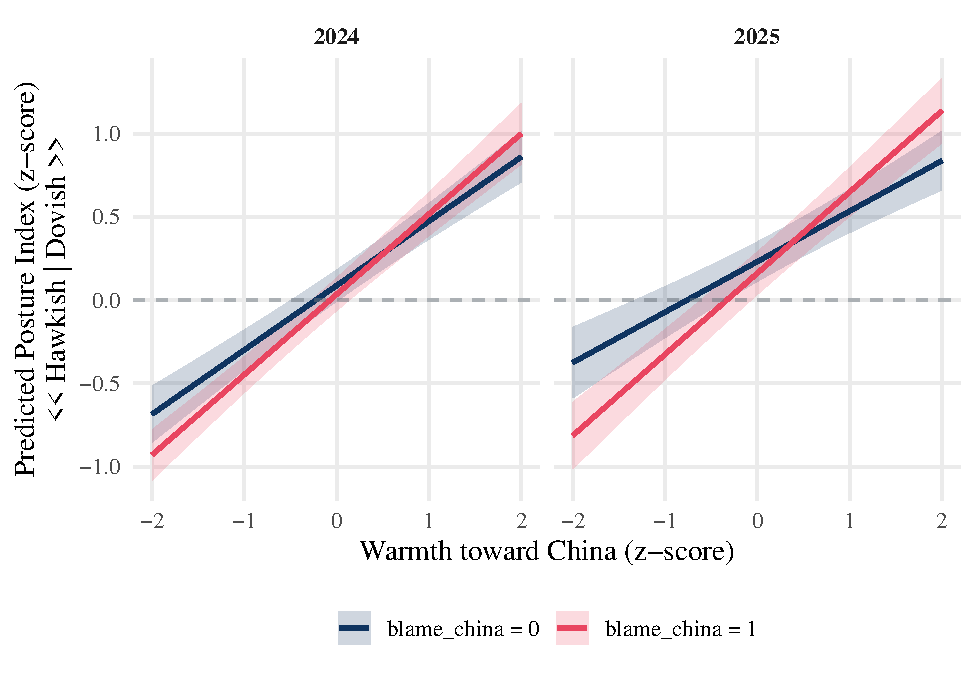
\includegraphics[width=0.95\textwidth]{figures/fig2a_posture_warmthXblame_byyear.pdf}
  \caption{Predicted foreign policy posture by warmth toward China and blame attribution, faceted by survey year. Lines represent survey-weighted OLS predictions with 95\% confidence intervals. The steeper slope under high blame illustrates the amplification interaction.}
  \label{fig:posture_interaction}
\end{figure}

\begin{table}[htbp]
\centering
\small
\caption{Survey-Weighted OLS: Foreign-Policy Posture Index on Warmth and Blame}
\label{tab:phase3_panel_a}
\label{tab:phase3_panel_b}

\begin{table}[htbp]
\begin{center}
\begin{tabular}{l c c c c c c}
\hline
 & A:2024 & A:2025 & A:Pool & B:2024 & B:2025 & B:Pool \\
\hline
(Intercept)            & $0.71^{***}$  & $0.38^{**}$  & $0.54^{***}$  & $0.54^{***}$  & $0.21$       & $0.38^{***}$  \\
                       & $(0.10)$      & $(0.14)$     & $(0.08)$      & $(0.10)$      & $(0.14)$     & $(0.08)$      \\
warmth\_z              & $0.39^{***}$  & $0.30^{***}$ & $0.35^{***}$  & $0.21^{***}$  & $0.19^{***}$ & $0.20^{***}$  \\
                       & $(0.03)$      & $(0.04)$     & $(0.03)$      & $(0.03)$      & $(0.04)$     & $(0.03)$      \\
blame\_china           & $-0.05$       & $-0.07$      & $-0.05$       & $-0.01$       & $-0.03$      & $-0.02$       \\
                       & $(0.04)$      & $(0.05)$     & $(0.03)$      & $(0.04)$      & $(0.05)$     & $(0.03)$      \\
party3Republican       & $-0.11$       & $-0.09$      & $-0.10^{*}$   & $-0.07$       & $-0.08$      & $-0.07$       \\
                       & $(0.06)$      & $(0.08)$     & $(0.05)$      & $(0.06)$      & $(0.08)$     & $(0.05)$      \\
party3Independent      & $-0.04$       & $-0.06$      & $-0.05$       & $0.01$        & $-0.02$      & $-0.00$       \\
                       & $(0.05)$      & $(0.06)$     & $(0.04)$      & $(0.05)$      & $(0.06)$     & $(0.04)$      \\
ideo5\_clean           & $-0.13^{***}$ & $-0.06$      & $-0.10^{***}$ & $-0.12^{***}$ & $-0.04$      & $-0.09^{***}$ \\
                       & $(0.02)$      & $(0.03)$     & $(0.02)$      & $(0.02)$      & $(0.03)$     & $(0.02)$      \\
educ\_college          & $-0.04$       & $0.01$       & $-0.02$       & $-0.03$       & $0.02$       & $-0.01$       \\
                       & $(0.04)$      & $(0.05)$     & $(0.03)$      & $(0.04)$      & $(0.04)$     & $(0.03)$      \\
age                    & $-0.00^{**}$  & $-0.00^{*}$  & $-0.00^{***}$ & $-0.00^{*}$   & $-0.00^{*}$  & $-0.00^{**}$  \\
                       & $(0.00)$      & $(0.00)$     & $(0.00)$      & $(0.00)$      & $(0.00)$     & $(0.00)$      \\
female                 & $0.01$        & $0.07$       & $0.04$        & $0.03$        & $0.06$       & $0.04$        \\
                       & $(0.04)$      & $(0.05)$     & $(0.03)$      & $(0.04)$      & $(0.04)$     & $(0.03)$      \\
race\_ethBlack         & $0.01$        & $-0.11$      & $-0.04$       & $0.00$        & $-0.12$      & $-0.05$       \\
                       & $(0.06)$      & $(0.08)$     & $(0.05)$      & $(0.06)$      & $(0.08)$     & $(0.05)$      \\
race\_ethHispanic      & $0.00$        & $-0.08$      & $-0.03$       & $0.01$        & $-0.07$      & $-0.02$       \\
                       & $(0.08)$      & $(0.08)$     & $(0.06)$      & $(0.08)$      & $(0.08)$     & $(0.06)$      \\
race\_ethAsian         & $-0.34^{**}$  & $-0.24^{*}$  & $-0.30^{***}$ & $-0.27^{*}$   & $-0.18$      & $-0.24^{**}$  \\
                       & $(0.11)$      & $(0.10)$     & $(0.08)$      & $(0.11)$      & $(0.11)$     & $(0.08)$      \\
race\_ethOther         & $-0.13$       & $0.07$       & $-0.04$       & $-0.10$       & $0.08$       & $-0.02$       \\
                       & $(0.07)$      & $(0.08)$     & $(0.05)$      & $(0.07)$      & $(0.08)$     & $(0.05)$      \\
newsint\_attn          & $-0.02$       & $0.05$       & $0.01$        & $-0.01$       & $0.06^{*}$   & $0.02$        \\
                       & $(0.02)$      & $(0.03)$     & $(0.02)$      & $(0.02)$      & $(0.03)$     & $(0.02)$      \\
exposure\_index        & $0.02$        & $-0.02$      & $0.00$        & $0.01$        & $-0.03$      & $-0.01$       \\
                       & $(0.03)$      & $(0.04)$     & $(0.03)$      & $(0.03)$      & $(0.04)$     & $(0.02)$      \\
warmth\_z:blame\_china & $0.10^{*}$    & $0.18^{***}$ & $0.13^{***}$  & $0.10^{*}$    & $0.15^{**}$  & $0.12^{***}$  \\
                       & $(0.05)$      & $(0.05)$     & $(0.03)$      & $(0.04)$      & $(0.05)$     & $(0.03)$      \\
factor(year)2025       &               &              & $0.11^{***}$  &               &              & $0.11^{***}$  \\
                       &               &              & $(0.03)$      &               &              & $(0.03)$      \\
behavior\_index\_z     &               &              &               & $0.30^{***}$  & $0.24^{***}$ & $0.28^{***}$  \\
                       &               &              &               & $(0.03)$      & $(0.03)$     & $(0.02)$      \\
\hline
Deviance               & $1913.21$     & $1203.12$    & $3141.58$     & $1783.39$     & $1148.17$    & $2956.09$     \\
Dispersion             & $0.75$        & $0.71$       & $0.74$        & $0.70$        & $0.68$       & $0.70$        \\
Num. obs.              & $2545$        & $1689$       & $4234$        & $2545$        & $1689$       & $4234$        \\
\hline
\multicolumn{7}{l}{\scriptsize{$^{***}p<0.001$; $^{**}p<0.01$; $^{*}p<0.05$}}
\end{tabular}
\caption{Panel A: blame\_china (Multi-Select, $\sim$49\%)}
\label{tab:phase3_panel_a}
\end{center}
\end{table}

% --- Panel B ---


\begin{table}[htbp]
\begin{center}
\begin{tabular}{l c c c c c c}
\hline
 & A:2024 & A:2025 & A:Pool & B:2024 & B:2025 & B:Pool \\
\hline
(Intercept)                 & $0.70^{***}$  & $0.39^{**}$  & $0.54^{***}$  & $0.55^{***}$  & $0.22$       & $0.38^{***}$  \\
                            & $(0.11)$      & $(0.14)$     & $(0.09)$      & $(0.11)$      & $(0.14)$     & $(0.09)$      \\
warmth\_z                   & $0.42^{***}$  & $0.37^{***}$ & $0.40^{***}$  & $0.25^{***}$  & $0.23^{***}$ & $0.24^{***}$  \\
                            & $(0.03)$      & $(0.03)$     & $(0.02)$      & $(0.03)$      & $(0.03)$     & $(0.02)$      \\
blame\_china\_alt           & $-0.06$       & $-0.09$      & $-0.06$       & $-0.09$       & $-0.09$      & $-0.08$       \\
                            & $(0.06)$      & $(0.08)$     & $(0.05)$      & $(0.06)$      & $(0.08)$     & $(0.05)$      \\
party3Republican            & $-0.10$       & $-0.06$      & $-0.08$       & $-0.05$       & $-0.05$      & $-0.05$       \\
                            & $(0.06)$      & $(0.08)$     & $(0.05)$      & $(0.06)$      & $(0.08)$     & $(0.05)$      \\
party3Independent           & $-0.03$       & $-0.04$      & $-0.03$       & $0.03$        & $-0.00$      & $0.02$        \\
                            & $(0.05)$      & $(0.06)$     & $(0.04)$      & $(0.05)$      & $(0.06)$     & $(0.04)$      \\
ideo5\_clean                & $-0.14^{***}$ & $-0.07^{*}$  & $-0.11^{***}$ & $-0.13^{***}$ & $-0.05$      & $-0.10^{***}$ \\
                            & $(0.02)$      & $(0.03)$     & $(0.02)$      & $(0.02)$      & $(0.03)$     & $(0.02)$      \\
educ\_college               & $-0.03$       & $0.03$       & $-0.01$       & $-0.03$       & $0.04$       & $-0.00$       \\
                            & $(0.04)$      & $(0.05)$     & $(0.03)$      & $(0.04)$      & $(0.04)$     & $(0.03)$      \\
age                         & $-0.00^{**}$  & $-0.00^{**}$ & $-0.00^{***}$ & $-0.00^{*}$   & $-0.00^{*}$  & $-0.00^{**}$  \\
                            & $(0.00)$      & $(0.00)$     & $(0.00)$      & $(0.00)$      & $(0.00)$     & $(0.00)$      \\
female                      & $0.02$        & $0.06$       & $0.04$        & $0.04$        & $0.06$       & $0.04$        \\
                            & $(0.04)$      & $(0.05)$     & $(0.03)$      & $(0.04)$      & $(0.05)$     & $(0.03)$      \\
race\_ethBlack              & $0.04$        & $-0.10$      & $-0.02$       & $0.02$        & $-0.10$      & $-0.03$       \\
                            & $(0.06)$      & $(0.09)$     & $(0.05)$      & $(0.06)$      & $(0.09)$     & $(0.05)$      \\
race\_ethHispanic           & $-0.01$       & $-0.06$      & $-0.03$       & $-0.00$       & $-0.05$      & $-0.02$       \\
                            & $(0.09)$      & $(0.08)$     & $(0.06)$      & $(0.08)$      & $(0.08)$     & $(0.06)$      \\
race\_ethAsian              & $-0.34^{**}$  & $-0.21$      & $-0.29^{***}$ & $-0.29^{*}$   & $-0.15$      & $-0.24^{**}$  \\
                            & $(0.12)$      & $(0.11)$     & $(0.09)$      & $(0.12)$      & $(0.11)$     & $(0.09)$      \\
race\_ethOther              & $-0.13$       & $0.09$       & $-0.04$       & $-0.10$       & $0.10$       & $-0.01$       \\
                            & $(0.07)$      & $(0.09)$     & $(0.06)$      & $(0.07)$      & $(0.08)$     & $(0.05)$      \\
newsint\_attn               & $-0.02$       & $0.04$       & $-0.00$       & $-0.01$       & $0.05$       & $0.01$        \\
                            & $(0.02)$      & $(0.03)$     & $(0.02)$      & $(0.02)$      & $(0.03)$     & $(0.02)$      \\
exposure\_index             & $0.02$        & $-0.01$      & $0.00$        & $0.00$        & $-0.01$      & $-0.00$       \\
                            & $(0.04)$      & $(0.04)$     & $(0.03)$      & $(0.03)$      & $(0.04)$     & $(0.03)$      \\
warmth\_z:blame\_china\_alt & $0.10$        & $0.18^{*}$   & $0.14^{**}$   & $0.06$        & $0.14$       & $0.10^{*}$    \\
                            & $(0.06)$      & $(0.08)$     & $(0.05)$      & $(0.06)$      & $(0.08)$     & $(0.05)$      \\
factor(year)2025            &               &              & $0.11^{***}$  &               &              & $0.11^{***}$  \\
                            &               &              & $(0.03)$      &               &              & $(0.03)$      \\
behavior\_index\_z          &               &              &               & $0.29^{***}$  & $0.25^{***}$ & $0.27^{***}$  \\
                            &               &              &               & $(0.03)$      & $(0.03)$     & $(0.02)$      \\
\hline
Deviance                    & $1815.59$     & $1133.97$    & $2973.47$     & $1695.54$     & $1080.92$    & $2801.44$     \\
Dispersion                  & $0.75$        & $0.70$       & $0.74$        & $0.70$        & $0.67$       & $0.70$        \\
Num. obs.                   & $2415$        & $1611$       & $4026$        & $2415$        & $1611$       & $4026$        \\
\hline
\multicolumn{7}{l}{\scriptsize{$^{***}p<0.001$; $^{**}p<0.01$; $^{*}p<0.05$}}
\end{tabular}
\caption{Panel B: blame\_china\_alt (Most Responsible, $\sim$11\%)}
\label{tab:phase3_panel_b}
\end{center}
\end{table}

\par\vspace{0.5ex}
{\footnotesize\textit{Notes.} Survey-weighted OLS. Dependent variable: standardized posture index (\texttt{posture\_z}). Panels A (columns 1--3) and B (columns 4--6) use the binary multi-select blame variable and the single-choice ``most responsible'' variable respectively, interacted with standardized warmth. Design-based standard errors in parentheses. * $p<0.05$, ** $p<0.01$, *** $p<0.001$.}
\end{table}

% ---------------------------------------------------------------------------
% 4.2 Issue-Level Tool Configuration
% ---------------------------------------------------------------------------
\subsection{Issue-Level Tool Configuration}
\label{sec:results_toolconfig}

Having established the warmth--blame interaction at the posture level, the analysis now examines whether this pattern is reflected in discrete tool configurations. Before turning to the multinomial results, a preliminary variance decomposition confirms that the two dependent variables capture largely distinct aspects of foreign-policy preferences. Tool configuration explains only 2.5\% of the weighted variance in general posture ($\eta^{2}=0.025$, $p<0.001$). S+A and Sanctions-only respondents occupy similar positions on the general posture spectrum (weighted means of $-0.24$ and $-0.14$ respectively), yet they differ sharply in tool composition.

Table~\ref{tab:phase4_estimands} reports predicted probabilities and blame-effect contrasts at one standard deviation below and above the warmth mean. Blame attribution is associated with a substantially higher probability of S+A classification at all warmth levels. Among cold respondents (warmth $= -1$ SD), the estimated $\hat{P}(\text{S+A})$ is 0.069 without blame and 0.363 with blame ($\Delta = +0.294$, $p < 0.001$). Among warm respondents ($+1$ SD), the corresponding figures are 0.044 and 0.350 ($\Delta = +0.306$, $p < 0.001$). By contrast, the blame effect on the Sanctions-only category is small and non-significant ($\Delta \approx 0$), consistent with blame channeling respondents into the combined S+A posture rather than a purely punitive stance.\footnote{The blame main effect on $P(\text{S+A})$ is robust to design-based inference (Supplementary Table~\ref{tab:app_design_mnl}); the warmth $\times$ blame interaction in tool composition is sensitive to it ($p = 0.240$ design-based vs.\ $p < 0.001$ model-based) and should be read as suggestive. The substantive IBC argument rests on the precise blame main effect, not the interaction.}

Figure~\ref{fig:toolconfig} displays the predicted probability of each tool configuration across \emph{warmth $\times$ blame} quadrants, making the selectivity of the blame effect visually apparent.

\begin{figure}[htbp]
  \centering
  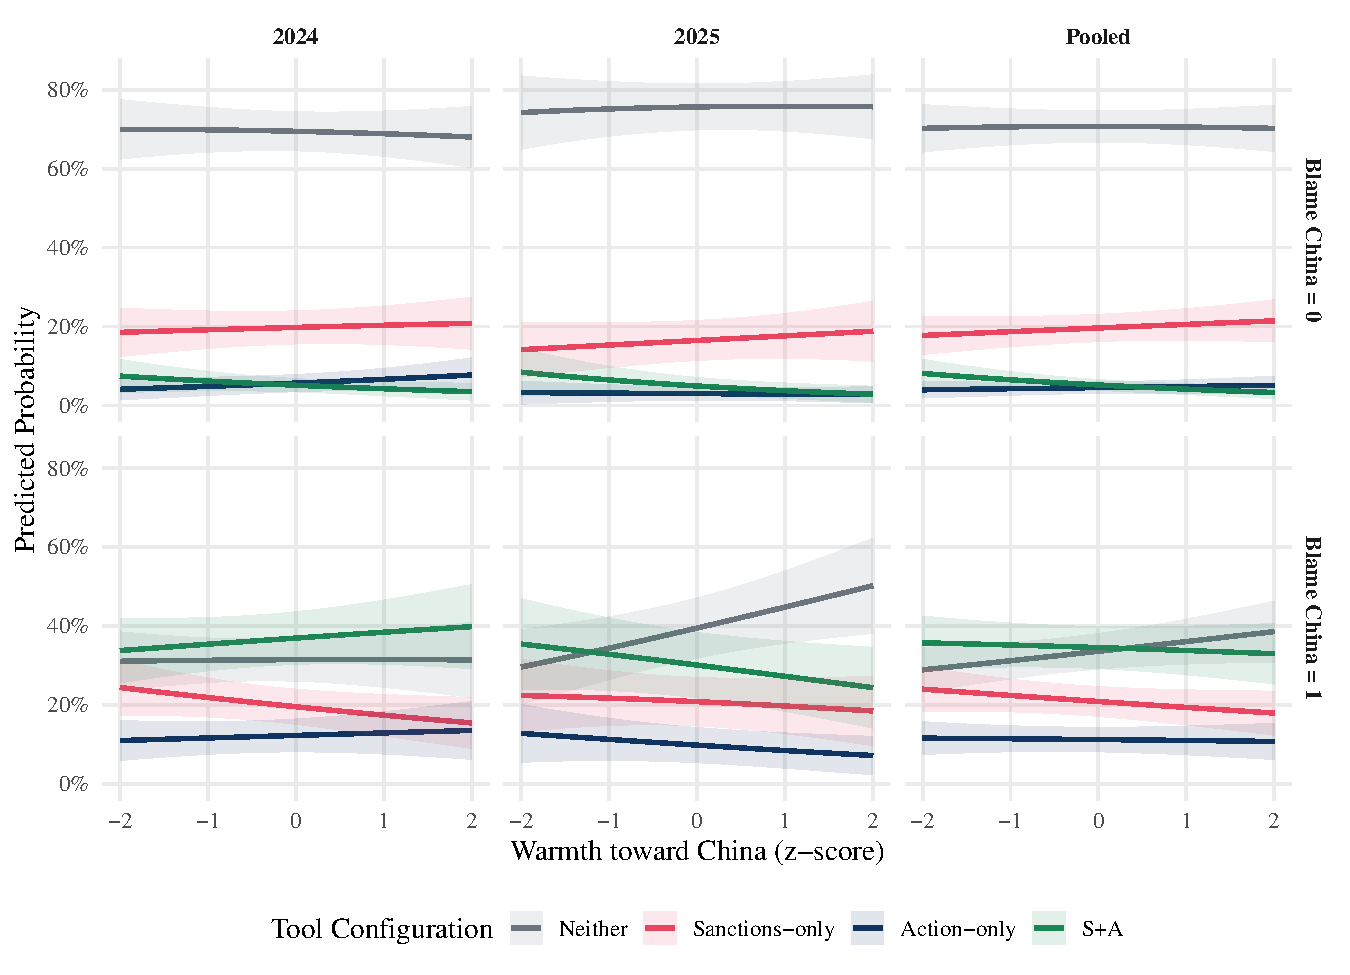
\includegraphics[width=0.85\textwidth]{figures/fig3_tool_config_warmthXblame.pdf}
  \caption{Predicted probability of each tool-configuration category by warmth $\times$ blame quadrant, from survey-weighted multinomial logit. Error bars show 95\% confidence intervals. Blame shifts respondents into S+A (sanctions plus cooperation) rather than Sanctions-only.}
  \label{fig:toolconfig}
\end{figure}

\begin{table}[htbp]
\centering
\small
\caption{Predicted Probabilities and Blame-Effect Contrasts: Multinomial Logit Estimates}
\label{tab:phase4_estimands}
\begin{table}[!h]
\centering
\caption{Phase 4 Key Estimands: Predicted Probabilities and Blame Effects}
\label{tab:phase4_estimands}
\centering
\begin{tabular}[t]{llll}
\toprule
Estimand & Estimate & SE & 95\% CI\\
\midrule
P\_SA\_w-1\_b0 & 0.0688 & 0.0112 & {}[0.0469, 0.0906]\\
P\_Sanctionsonly\_w-1\_b0 & 0.1907 & 0.0201 & {}[0.1513, 0.2301]\\
P\_SA\_w-1\_b1 & 0.3632 & 0.0287 & {}[0.3070, 0.4194]\\
P\_Sanctionsonly\_w-1\_b1 & 0.2229 & 0.0212 & {}[0.1813, 0.2645]\\
P\_SA\_w+1\_b0 & 0.0437 & 0.0073 & {}[0.0293, 0.0581]\\
P\_Sanctionsonly\_w+1\_b0 & 0.2097 & 0.0209 & {}[0.1688, 0.2507]\\
P\_SA\_w+1\_b1 & 0.3495 & 0.0321 & {}[0.2866, 0.4124]\\
P\_Sanctionsonly\_w+1\_b1 & 0.1930 & 0.0229 & {}[0.1482, 0.2379]\\
Dpp\_SA\_w-1 & 0.2944 & 0.0248 & {}[0.2458, 0.3430]\\
Dpp\_Sonly\_w-1 & 0.0322 & 0.0203 & {}[-0.0075, 0.0719]\\
Dpp\_SA\_w+1 & 0.3058 & 0.0289 & {}[0.2492, 0.3624]\\
Dpp\_Sonly\_w+1 & -0.0167 & 0.0211 & {}[-0.0581, 0.0247]\\
\bottomrule
\end{tabular}
\end{table}

\par\vspace{0.5ex}
{\footnotesize\textit{Notes.} Survey-weighted multinomial logit. Predicted probabilities evaluated at warmth $= \pm 1$ SD; contrasts ($\Delta_{\text{pp}}$) are predicted-probability differences between blame $= 1$ and blame $= 0$ at the indicated warmth level. Standard errors are Hessian-based (model-based). Reference category: Neither.}
\end{table}

A potential concern is that the S+A pattern reflects acquiescent response style---a general tendency to endorse survey items---rather than genuine policy differentiation \citep{krosnick_response_1991}. This is addressed by controlling for an endorsement-count measure that attenuates the S+A blame effect by approximately 38\% (from $\Delta = 0.306$ to $\Delta = 0.191$ among warm respondents). Such a substantial reduction indicates that acquiescent response style accounts for a meaningful share of the raw effect. Nevertheless, the qualitative pattern---blame increases S+A, not Sanctions-only---remains intact, and the specificity test in Section~\ref{sec:results_specificity} provides further evidence against a pure response-style explanation (Supplementary Table~\ref{tab:app_acquiescence}). A placebo test replacing the dependent variable with a sanctions $\times$ international-cooperation composite (theoretically unrelated to specific U.S.-China collaboration) does not support tool-specificity. This limitation is revisited in Section~\ref{sec:discussion}.

% ---------------------------------------------------------------------------
% 4.3 Testing Issue-Bounded Conditionality Across Scenarios
% ---------------------------------------------------------------------------
\subsection{Testing Issue-Bounded Conditionality Across Scenarios}
\label{sec:results_specificity}

The preceding analyses show that blame shifts respondents into the S+A configuration. However, does this classification reflect issue-bounded conditionality, or a general willingness to cooperate with China? The specificity test addresses this by comparing the S+A--versus--S-only contrast across eight scenarios. If the contrast appears only on the fentanyl target probe and not on the seven boundary probes, the classification captures something specific to that issue rather than a diffuse disposition.

Table~\ref{tab:probe_map} maps each scenario to the scope conditions developed in Section~\ref{sec:theory_ibc}. The assignment of scope conditions to probes is theory-derived: the two conditions (problem structure and tool structure) were specified in Section~\ref{sec:theory_ibc} prior to any analysis of the probe battery, and the probe-to-condition mapping follows directly from the theoretical definitions. The probes were not assigned to conditions based on the pattern of the results; the expected direction ($\approx 0$ vs.\ $> 0$) was fixed before estimation. The target probe (probe $d$, \emph{Fentanyl cooperation}) is the only scenario in which both conditions are fully satisfied. The three security probes ($a$--$c$) violate the \emph{tool-structure} condition: military instruments are relationship-ending rather than bounded, so the framework predicts reversion to a unidimensional confrontational posture. The four non-military probes ($e$--$h$) violate the \emph{problem-structure} condition: they describe steady-state policy questions without a salient crisis, traceable blame, or compliance-dependent resolution. In all seven boundary cases, the framework predicts no amplified S+A-minus-S-only contrast.

\begin{table}[!h]
\centering
\small
\caption{Eight-Probe Battery: Domain, Scope Conditions, and Expected Direction}
\label{tab:probe_map}
\begin{tabular}{cllcc}
\toprule
Probe & Scenario & Domain & Scope condition violated & Expected $\Delta$ \\
\midrule
$a$ & Taiwan military action & Security & Tool structure & $\approx 0$ \\
$b$ & U.S.-China military collision & Security & Tool structure & $\approx 0$ \\
$c$ & Third-party military collision & Security & Tool structure & $\approx 0$ \\
$d$ & \textbf{Fentanyl cooperation} & \textbf{Health} & \textbf{None (target)} & $\boldsymbol{> 0}$ \\
$e$ & Resuming adoptions from China & Cultural & Problem structure & $\approx 0$ \\
$f$ & Halting electronics sales & Economic & Problem structure & $\approx 0$ \\
$g$ & Chinese student scholarships & Cultural & Problem structure & $\approx 0$ \\
$h$ & Pandas returning to U.S. zoos & Cultural & Problem structure & $\approx 0$ \\
\bottomrule
\end{tabular}
\end{table}

Table~\ref{tab:phase5_contrasts} reports the core results, where each entry is the adjusted mean difference in opinion-change scores between S+A and Sanctions-only respondents for that probe. The target contrast is $\Delta_d = +0.282$ ($p = 0.002$). In substantive terms, S+A respondents score 0.28 scale points higher than S-only respondents on the fentanyl-cooperation probe (on a 1--7 scale), after controlling for demographics, ideology, political attention, and exposure. None of the seven boundary probes achieves significance individually, and the composite boundary mean is small and non-significant ($\bar{\Delta}_{\text{boundary}} = +0.042$, $p = 0.337$).

The omnibus divergence---the difference between the target contrast and the composite boundary mean---is $+0.240$ ($p = 0.008$), consistent with a concentration of the S+A effect on the fentanyl cooperation dimension. A TOST equivalence test confirms that the composite boundary mean is negligibly small ($p = 0.009$). It indicates that S+A respondents do not differ meaningfully from S-only respondents on non-fentanyl scenarios. Figure~\ref{fig:panorama} presents the results visually, contrasting the S+A--versus--S-only adjusted means for each probe. Probe $d$ is the only probe with a significant and substantively large contrast.

\begin{figure}[htbp]
  \centering
  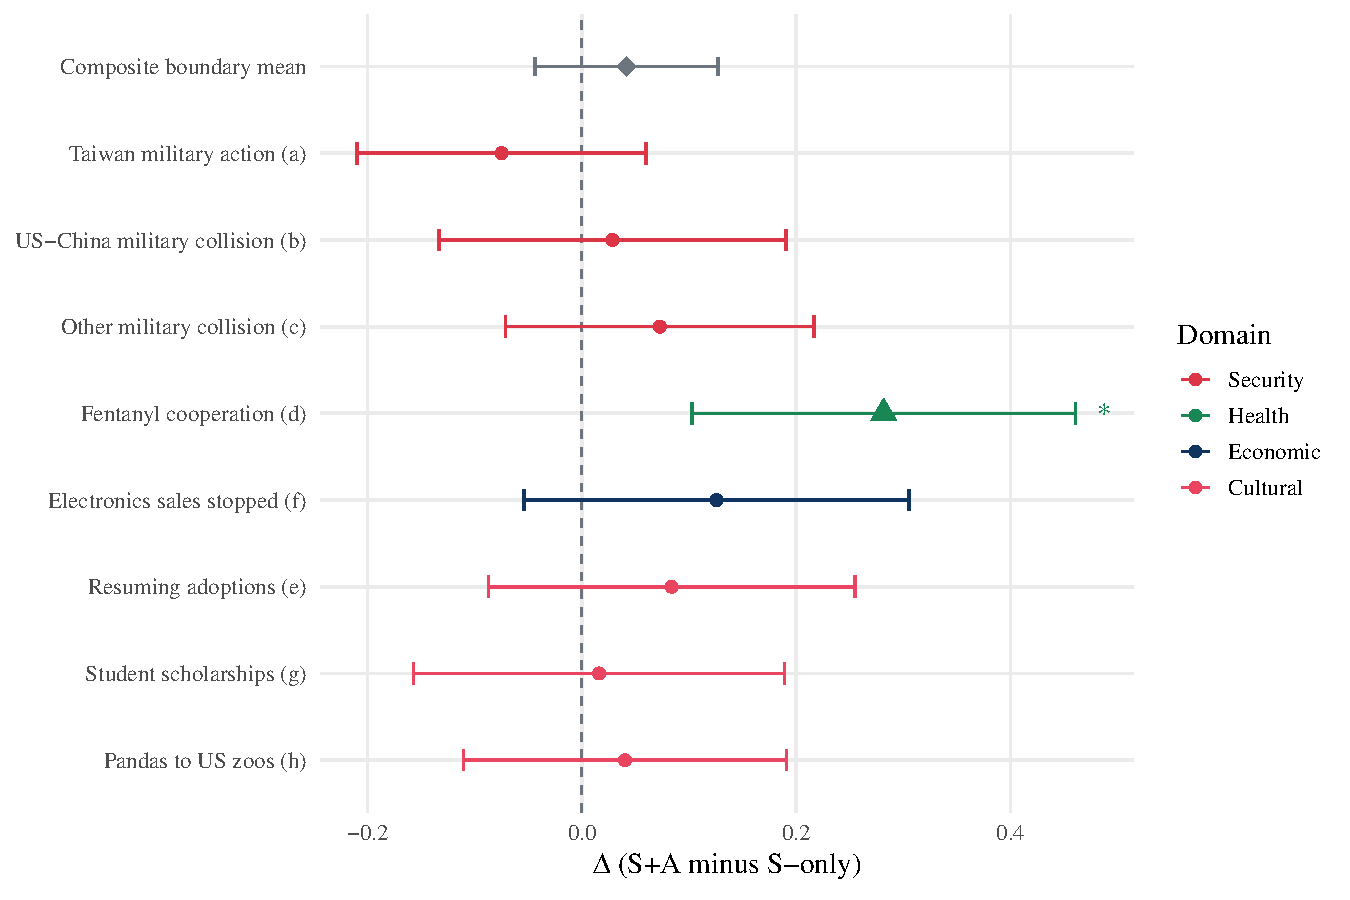
\includegraphics[width=0.95\textwidth]{figures/fig4_probes_panorama.pdf}
  \caption{Adjusted mean differences in opinion-change scores (S+A minus S-only, in 1--7 scale-point units) for eight scenario probes. Probe $d$ (fentanyl cooperation) is the target; probes $a$--$c$ and $e$--$h$ are boundary probes. Points show estimated $\Delta$ with 95\% confidence intervals. The dashed vertical line marks zero. Only the target probe is significant, consistent with issue-bounded conditionality.}
  \label{fig:panorama}
\end{figure}

\begin{table}[htbp]
\centering
\small
\caption{Issue-Specificity Test: Adjusted Mean Differences in Opinion-Change Scores (S+A minus S-only)}
\label{tab:phase5_contrasts}
\begin{table}[!h]
\centering
\caption{Phase 5: Panorama Discrimination Contrasts (S+A minus S-only)}
\label{tab:phase5_contrasts}
\centering
\begin{tabular}[t]{lllll}
\toprule
Contrast & Estimate & SE & CI & p\_value\\
\midrule
Delta\_d (target: Fentanyl cooperation) & 0.2817 & 0.0913 & {}[0.1027, 0.4607] & 0.002**\\
Composite boundary mean(Delta\_others) & 0.0417 & 0.0434 & {}[-0.0435, 0.1269] & 0.337\\
Omnibus divergence (Delta\_d - composite) & 0.2400 & 0.0910 & {}[0.0616, 0.4184] & 0.008**\\
TOST equivalence (eps=0.145) & 0.0417 & 0.0434 & +/- 0.145 & 0.009**\\
\bottomrule
\end{tabular}
\end{table}

\par\vspace{0.5ex}
{\footnotesize\textit{Notes.} Stacked OLS with respondent clustering. Each row is $\Delta_k$ = adjusted mean difference in opinion-change score between S+A and Sanctions-only respondents for probe $k$, on a 1--7 scale. Controls: demographics, ideology, political attention, and exposure index. * $p < 0.05$; ** $p < 0.01$; *** $p < 0.001$.}
\end{table}

These results are robust across multiple specifications. Pairwise divergence tests---comparing $\Delta_d$ against each boundary probe individually, with Benjamini--Hochberg false discovery rate correction \citep{benjamini_controlling_1995}---confirm that the target probe is significantly larger than two of seven boundary probes at the BH-FDR adjusted $\alpha = 0.05$ level (four of seven at the unadjusted level), and directionally larger than all seven (Supplementary Table~\ref{tab:app_divergence}). An alternative specification using continuous $\hat{P}(\text{S+A})$ predicted probabilities in place of the binary classifier yields estimates consistent in sign and magnitude (Supplementary Table~\ref{tab:app_phat}). In sum, the concentration of the S+A contrast on the fentanyl probe, with near-zero boundary effects, is consistent with issue-bounded conditionality rather than a generalized cooperative disposition.

% ---------------------------------------------------------------------------
% 4.4 Descriptive Mechanism Evidence: Leverage vs. Normative Readings
% ---------------------------------------------------------------------------
\subsection{Interpreting the S+A Configuration: Descriptive Mechanism Evidence}
\label{sec:results_mechanism}

Section~\ref{sec:theory_ibc} advanced \emph{bounded instrumental logic}---leverage---as the working hypothesis for why blame conditions warmth, and flagged a normative alternative in which sanctions plus action simply encode the ``right'' response to adversary transgression. A cross-sectional design cannot adjudicate directly between these mechanisms, since both predict elevated joint endorsement of the two items. What the survey can do is report, descriptively, whether S+A respondents view the bilateral channel in ways consistent with the leverage reading---whether they treat China as an actor whose behavior they are trying to move, rather than as an opponent to be punished expressively. Four items from the instrument are used to probe this: whether respondents name the Chinese government as primarily responsible for fixing the problem; whether they endorse improved international cooperation as part of the solution; whether they endorse health and justice collaborations; and where they place China on a seven-point competitive--cooperative scale. Table~\ref{tab:mechanism_descriptive} reports survey-weighted comparisons between S+A and S-only respondents on these four items, pooled across the 2024 and 2025 waves.\footnote{The four items are available in both waves (PAXS0003 and PAXS0004); the seven-point competitive--cooperative scale is labeled \texttt{q14\_b} in the 2024 instrument and \texttt{q13\_b} in the 2025 instrument but uses identical wording and response options.}

\begin{table}[!h]
\centering
\small
\caption{Descriptive Mechanism Comparisons: S+A vs. Sanctions-only Respondents}
\label{tab:mechanism_descriptive}
\begin{tabular}{p{0.42\textwidth}ccc}
\toprule
Item & S+A & S-only & Difference (95\% CI) \\
\midrule
\% naming Chinese government as primarily responsible for fixing (q9) & 10.0\% & 2.8\% & +7.2 pp (5.0, 9.4) \\
\% endorsing improved international cooperation (q10\_1) & 77.2\% & 38.1\% & +39.0 pp (34.8, 43.3) \\
\% endorsing health and justice collaborations (q10\_5) & 45.3\% & 29.1\% & +16.3 pp (11.8, 20.7) \\
Mean competitive--cooperative rating, 1--7 (q13\_b / q14\_b) & 2.04 & 2.55 & $-$0.51 ($-$0.66, $-$0.36) \\
\bottomrule
\end{tabular}
\\[0.5em]
\footnotesize \textit{Notes.} Pooled sample of S+A and Sanctions-only respondents across the 2024 and 2025 waves ($n = 2{,}071$; 1{,}083 S+A, 988 S-only). Entries are survey-weighted proportions (rows 1--3) and a weighted mean (row 4). Confidence intervals are based on linearization standard errors. Positive differences favor the S+A group; a negative difference on row 4 indicates that S+A respondents place China closer to the ``competitive'' end of the 1--7 scale than S-only respondents.
\end{table}

Three features of the comparison support the leverage reading. First, S+A respondents are more than three times as likely as S-only respondents to name the Chinese government as the group most responsible for \emph{fixing} the problem (10.0\% vs.\ 2.8\%, a 7.2-point gap). This is the strongest single indication that ``requiring action by China'' reads, for the S+A group, as the \emph{remedy} they are trying to extract rather than as a second punitive demand layered on top of sanctions: the Chinese state is cast as the agent whose compliance resolves the crisis, not merely as the agent who caused it. Second, S+A respondents endorse the international-cooperation and health-collaboration items at substantially higher rates---77.2\% vs.\ 38.1\% for improved international cooperation, and 45.3\% vs.\ 29.1\% for health and justice collaborations. Their general orientation toward the fentanyl problem is visibly collaborative rather than punitive; in their adjacent answers they look like people who think the solution runs through engagement. Third, this collaborative orientation is \emph{not} rooted in a benign view of the bilateral relationship. On the seven-point competitive--cooperative scale, S+A respondents place China at 2.04, about half a point \emph{more} competitive than the 2.55 mean among S-only respondents. The combination is exactly what a leverage logic would predict: S+A respondents are realist---even a touch more hard-eyed than S-only respondents---about China's current behavior, yet they endorse engagement-shaped instruments because they see compliance as the objective rather than rupture. A group that already believed the relationship was amicable would have little reason to pair sanctions with demands in the first place.

These patterns are emphatically descriptive, not causal. They do not identify a mechanism---they characterize the orientation of the S+A group on adjacent items. A respondent who answers the four items this way could still be motivated by normative considerations rather than instrumental ones; the items do not directly tap the citizen's reasoning process. What the comparison does establish is whether the mechanism story is \emph{coherent}: whether S+A respondents look, in their other answers, like people pursuing leverage or like people cheering for punishment. The Discussion returns to what the cross-sectional design can and cannot settle and sketches an experimental design that could adjudicate the question directly.

% ===========================================================================
% 5. DISCUSSION AND CONCLUSION
% ===========================================================================
\section{Discussion and Conclusion}
\label{sec:discussion}

% ¶1 — Core Finding and Theoretical Implication
General foreign-policy posture and issue-level tool preferences toward China operate as partially independent levels of opinion, and crisis-specific blame is associated with a reorganization of the relationship between them. Blame for the fentanyl crisis does not push warm respondents toward confrontation. It is associated with a distinctive mixed configuration in which coercive and cooperative tools coexist within a bounded policy domain. This two-level structure challenges the assumption, implicit in much of the image-theory and threat-perception literature, that affective orientation toward a rival state determines policy preferences in a unidimensional fashion. When a domestic crisis is attributed to a foreign actor, citizens appear to differentiate not only between policy objectives, as the ``pretty prudent public'' tradition has long argued, but also between instruments. The present results are more consistent with a reading in which some coercive tools are compatible with ongoing engagement than with one in which they signal relationship rupture.

% ¶2 — How Strong Is the Evidence?
Two features of the results warrant particular interpretive caution, and both acquire a different weight once the S+A configuration is read as compliance-seeking leverage rather than as cooperation in the relational-trust sense developed in Section~\ref{sec:theory_ibc}. First, a placebo test using an alternative tool pairing (sanctions combined with \emph{improved international cooperation}, in place of China-specific fentanyl cooperation) produced a blame-driven shift of comparable magnitude. A formal comparison of the two blame contrasts---$\Delta_{\text{pp}}$(S+A) from the main specification against $\Delta_{\text{pp}}$(Sanctions+IntlCoop) from the placebo---yields a difference of $-0.029$ ($SE = 0.095$, $t = -0.31$, $p = 0.758$; Supplementary Table~\ref{tab:app_placebo_contrast}). The two contrasts are statistically indistinguishable. Read narrowly as a failure of tool-level specificity, this finding would be corrosive: it would suggest that any cooperative-sounding item pairs similarly well with sanctions, and the S+A configuration might then reflect a generic ``sanctions plus something nice'' response pattern. Read through the leverage framework, however, the placebo is considerably less damaging. Both pairings are engagement-compatible pressure packages: both couple a coercive instrument with a cooperative one, and both presuppose an ongoing channel through which pressure can be applied and compliance extracted. That they move in parallel with blame is consistent with the idea that blame activates a \emph{leverage orientation} that does not discriminate finely between specific cooperative items. What the placebo cannot do, in either reading, is dislodge the domain-level concentration documented in Section~\ref{sec:results_specificity}: the eight-probe panorama showed that the S+A contrast is confined to the fentanyl cooperation scenario and is negligible across military, economic, and cultural domains. The framework's central claim is domain-concentration, not tool-specificity, and that claim survives the placebo.

Second, controlling for acquiescent response style attenuates the S+A blame effect by approximately 38\%. The uncorrected estimates should therefore be treated as an upper bound and the acquiescence-adjusted estimates as a conservative floor. Even at the floor, the qualitative pattern persists: blame is associated with an increase in the S+A configuration, not with an increase in Sanctions-only. Under the leverage reading, what the acquiescence correction removes is diffuse willingness to agree with surveyed items; what remains is the part of the S+A pattern that cannot be explained by endorsement style alone, and it is this residual---not the raw coefficient---that carries the framework's claim. If this pattern generalizes beyond the present sample, it also carries a methodological implication for the broader public-opinion literature: survey-based studies of attitudes toward China that do not account for endorsement tendency may overstate the prevalence of mixed or cooperative preference configurations.

% ¶3 — Limitations and Interpretive Boundaries
The evidence supports the claim that warmth and blame jointly structure both posture and tool composition, and that the resulting mixed configuration is domain-specific. It does not establish causality. The design uses repeated cross-sections, and the observed associations may reflect unmeasured confounders or reverse causation. The specificity test reduces the plausibility of a generalized acquiescence account but cannot distinguish bounded instrumental logic from domain-specific social desirability, the possibility that respondents endorse fentanyl cooperation because prevailing media frames make it the expected complement to sanctions, not because of a genuinely differentiated preference structure. The inclusion of the standardized posture index as a control variable conditions on a post-treatment covariate, meaning that the tool-composition estimates (Step~2) capture within-posture effects over total effects. The framework is tested on a single bilateral case and across two waves that bracket a substantial change in the elite framing environment---the 2025 wave was fielded after the Trump administration's fentanyl-related tariffs but before the later-2025 Busan bilateral agreement. The conditional pattern appears stronger in 2025 (Supplementary Table~\ref{tab:app_within_wave}), which is consistent with elite framing that tied punitive instruments to counternarcotics cooperation, though the design cannot adjudicate between this account and other political shifts during the intervening year. Whether issue-bounded conditionality generalizes to other crisis domains, other bilateral relationships, or different elite-framing environments remains an open question. Standard errors are model-based rather than design-based, which may understate uncertainty if the assumed variance structure is misspecified. %Finally, the design controls for partisanship but lacks statistical power for three-way interactions. Whether Democrats and Republicans exhibit conditionality to the same degree is a question the present data cannot resolve.

% ¶4 — Implications for Understanding Public Opinion and U.S.–China Relations
Public opinion on China is more internally differentiated than aggregate favorability polls indicate \citep{li_more_2021}, with three implications for scholars and practitioners. The domestic political space for issue-specific engagement may be wider than hawk--dove framings imply. A public hostile toward China will not necessarily reject cooperative initiatives; what appears to matter is whether cooperation is tied to a concrete, accountable objective---stemming the fentanyl supply---rather than framed as a general diplomatic concession. That latitude is sharply bounded, though: support for cooperation does not transfer across issue areas. Extrapolating from public willingness to cooperate on fentanyl to an appetite for broader engagement on trade, technology, or military confidence-building would misread the data. Blame attribution does not function as a simple barrier to cooperation but as a structuring condition: citizens who blame China most intensely are also, conditional on warmth, the most likely to endorse the mixed sanctions-and-cooperation configuration. This is consistent with the logic of issue publics, in which crisis salience activates a subgroup with distinctive, issue-bounded preferences. ``Tough on China'' rhetoric and issue-specific cooperation are not zero-sum in the public mind. The former may help make the latter politically acceptable when cooperation is tied to a concrete and accountable objective.

% ¶5 — Return to Puzzle and Answer
%When a lethal domestic crisis is attributed to a foreign rival, does the public demand confrontation, or can it sustain a more differentiated response? In a nutshell, the answer is conditional given the evidence presented here. Citizens can simultaneously endorse coercive and cooperative tools, but only within the specific policy domain activated by crisis blame, and not as a generalized orientation toward the bilateral relationship.

% ¶6 — Future Research
Several extensions would strengthen the framework. Panel data tracking the same respondents over time would clarify whether issue-bounded conditionality is a stable preference configuration or a transient response to crisis salience. Experimental manipulation of blame attribution---randomly assigning respondents to receive information attributing the fentanyl crisis to China, to domestic actors, or to diffuse causes---would permit causal identification of the blame mechanism that the present cross-sectional design can only suggest, and could also adjudicate between the leverage and normative readings of the S+A configuration by measuring whether exogenous shifts in blame move cooperative-item endorsement in the direction leverage predicts. Testing the framework on other bilateral crises that plausibly satisfy the scope conditions, such as U.S.-China cooperation on climate change or technology governance, would establish whether issue-bounded conditionality is a general feature of public opinion under crisis attribution or a phenomenon unique to the case of synthetic opioids. Finally, on the estimation side, hierarchical or multilevel specifications that allow random intercepts for respondents and for scenario probes would be a natural methodological extension of the stacked-OLS design used here, particularly for analyses that aim to partition variance in S+A preferences across individuals, issues, and waves.

% ===========================================================================
% 6. REFERENCES
% ===========================================================================
\printbibliography
\end{document}
